%
% $RCSfile: ontology_framework.tex,v $
%
% Copyright (c) 2001-2004. Christian Heller. All rights reserved.
%
% No copying, altering, distribution or any other actions concerning this
% document, except after explicit permission by the author!
% At some later point in time, this document is planned to be put under
% the GNU FDL license. For now, _everything_ is _restricted_ by the author.
%
% http://www.cybop.net
% - Cybernetics Oriented Programming -
%
% http://www.resmedicinae.org
% - Information in Medicine -
%
% @author Christian Heller <christian.heller@tuxtax.de>
%

\subsection{Ontology Framework}
\label{ontology_framework_heading}

When placing the translators of figure \ref{translator_classes_figure} into the
greater system architecture context, a \emph{System Ontology} as shown in
figure \ref{system_ontology_figure} may be retrieved. It contains the new
\emph{Translator} as sub class of \emph{Region}, input/ output devices as sub
class of \emph{Block}, \emph{Module} (\emph{Application}) and \emph{User} as sub
class of \emph{System} and further parts which are not the topic of this paper.
For the ease of understanding, the biological counterparts have been added on
the right side of the figure.\\
Specialized translators may be derived as sub class of the one shown in figure
\ref{system_ontology_figure}.

\begin{figure}[ht]
    \begin{center}
        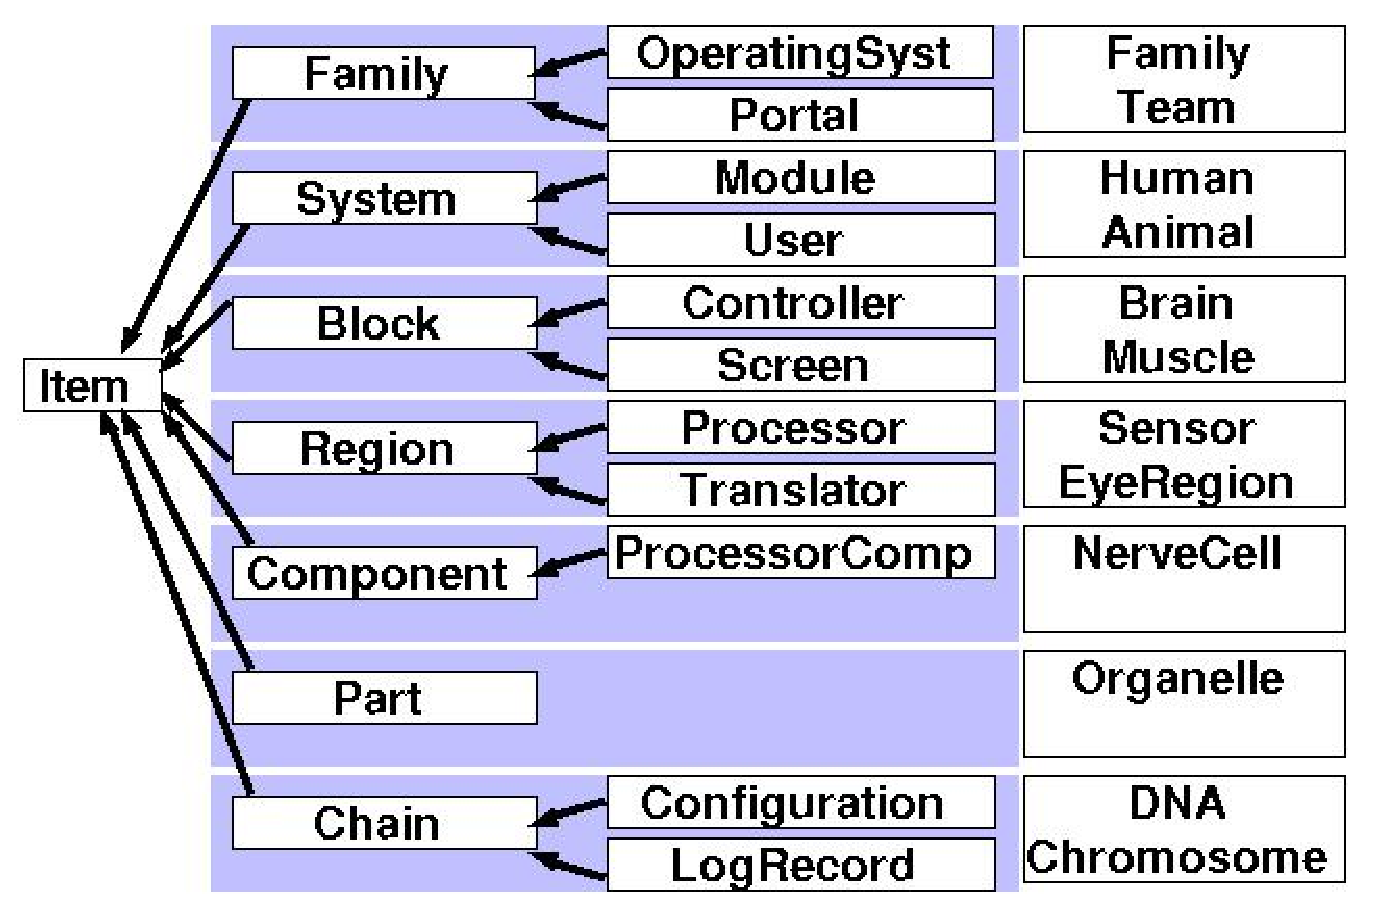
\includegraphics[scale=0.3]{vector/system_ontology.eps}
        \caption{System Ontology}
        \label{system_ontology_figure}
    \end{center}
\end{figure}

To complete the list of important ontology models, figure \ref{basic_ontology_figure}
gives an overview of language-integrated types (commonly called \emph{Primitives}).
And as a matter of fact: All typecasted programming languages already contain an
\emph{Ontology}!
These primitives represent the lowest layer in an ontology or in other words, the
last level of abstraction in software. That is also where \emph{Terminologies}
(that are mostly mentioned in conjunction with ontologies) come in. Basically,
these are sorted collections of terms (strings) but not further elaborated here.

\begin{figure}[ht]
    \begin{center}
        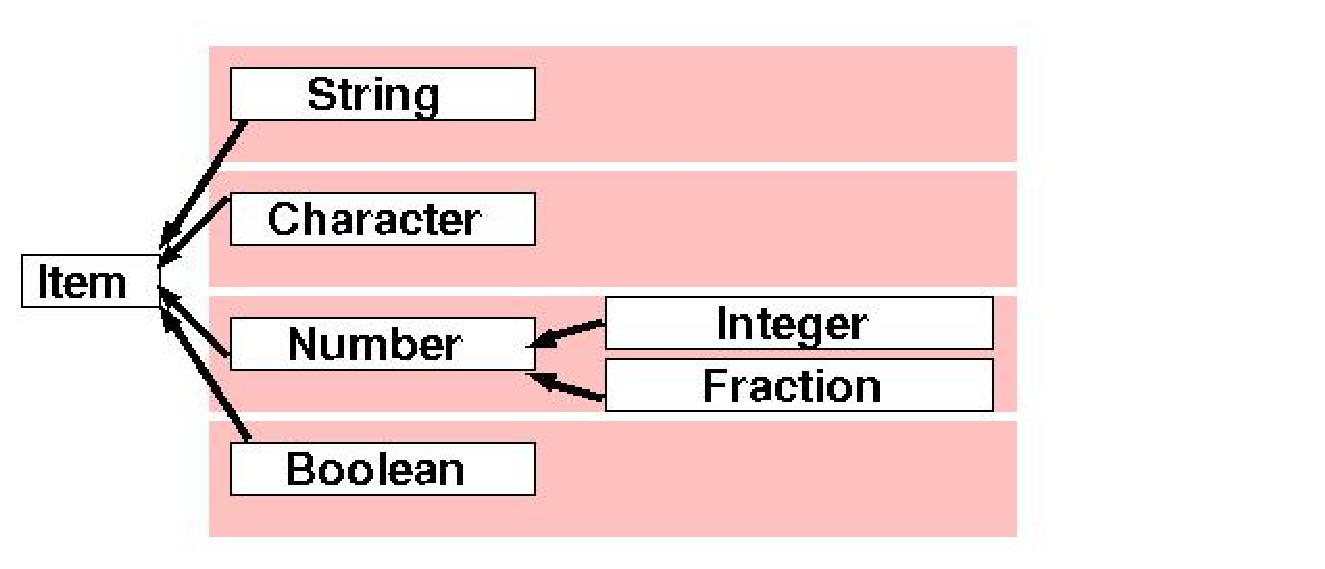
\includegraphics[scale=0.4]{vector/basic_ontology.eps}
        \caption{Basic (Language) Ontology}
        \label{basic_ontology_figure}
    \end{center}
\end{figure}

Putting the three ontologies \emph{Basic}, \emph{Model} and \emph{System} that were
introduced in this paper together, results in the CYBOP architecture of figure
\ref{ontology_framework_figure}. All ontologies base on the \emph{Language Ontology}.
A system built after the \emph{System Ontology} model (in this paper the example
of an \emph{Electronic Health Record} application) may access one ore more
\emph{Model Ontologies} (in the example the health record domain model).
All dependencies are unidirectional.

\begin{figure}[ht]
    \begin{center}
        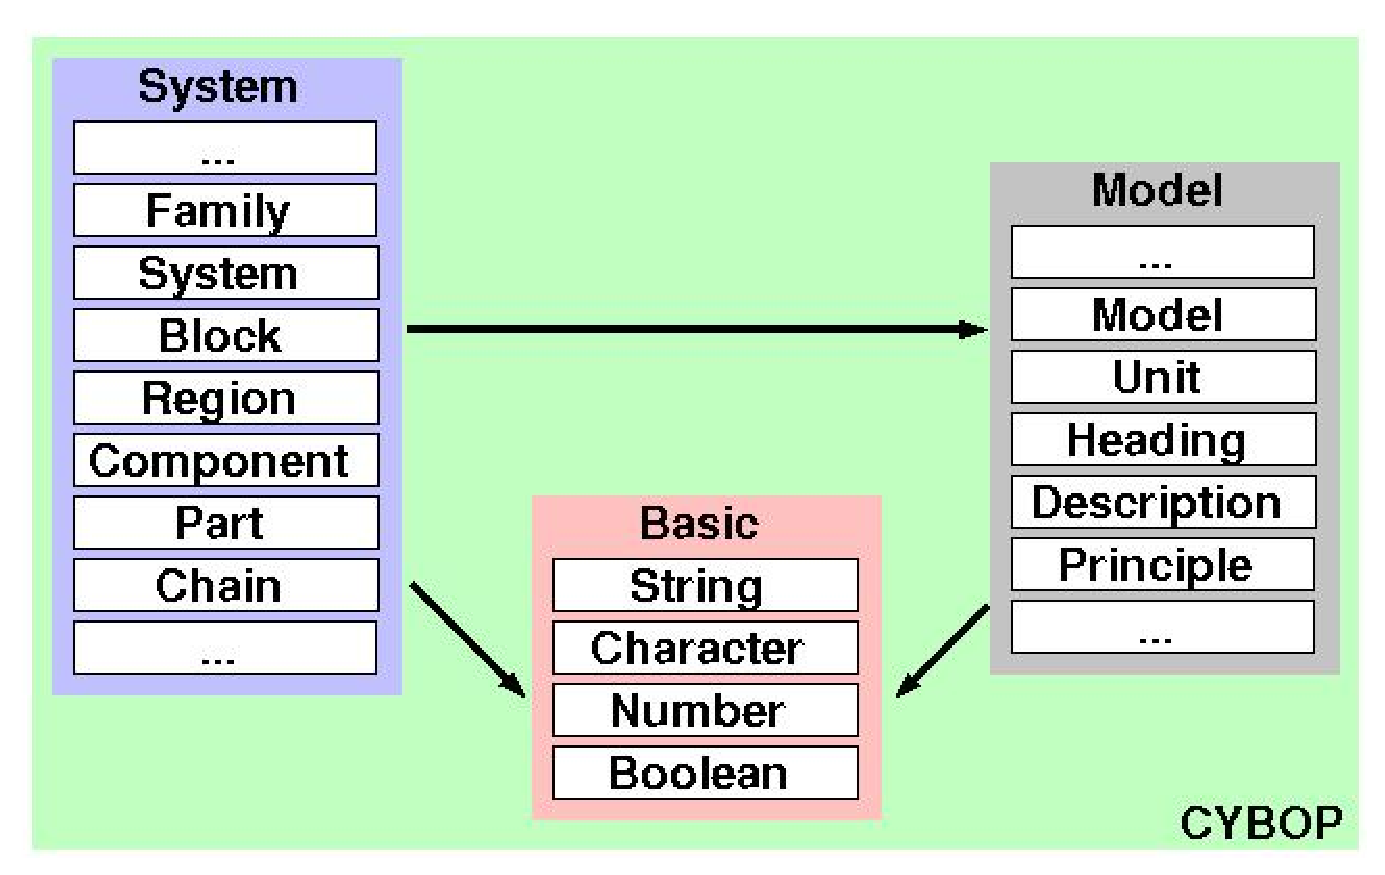
\includegraphics[scale=0.3]{vector/ontology_framework.eps}
        \caption{CYBOP Ontology Framework}
        \label{ontology_framework_figure}
    \end{center}
\end{figure}

